\section{Einleitung}
\label{sec:introduction}

\subsection{\"Uber den Autor}
\label{sec:author}

Der Autor entstammt einer alteingesessenen, Westberliner Familie und ist irgendwann in den 80ern geboren.
So wichtig dieser Lokalpatriotismus dem Autor auch ist, so stark bef\"urwortet er und bewegt ihn auch das Zusammenwachsen mit dem \"ubrigen Ostdeutschland.
Ostberliner und Brandenburger waren seit der fr\"uhen Jugend immer in gro{\ss}er Zahl im Freundeskreis vertreten.

Die Mauer ist tats\"achlich nur eine sehr d\"unne Erinnerung.
Dennoch waren die Grenzkontrollen im Familienurlaub immer sehr beeindruckend und wurden auch auf den mit dem Bruder gezeichneten Spielstra{\ss}en z.T. verarbeitet.
In Sachsen gab es auch einen Ableger der Familie.
Dort war Onkel Kurt's Modelleisenbahnanlage legend\"ar, war sie szenisch doch unglaublich ausgebaut und zudem praktisch, an die Wand klappbar untergebracht.
In der engen Familie selbst hatten wir auch mehrere Anlagen, siehe pers\"onlicher Appendix, Kap.~\ref{sec:personalAppendix}.
Diese gingen nur sp\"arlich \"uber das Stadium der Gleisw\"uste hinaus.
Pl\"ane zur Ausgestaltung gab es immer viele, realisiert wurden aber nur einige H\"auseraufstellungen sowie aufgeklebte Stra{\ss}en.
Spielspa{\ss} haben sie trotzdem viel geboten.

Sp\"atestens im 14. Lebensjahr muss das Interesse an der Modellbahn verloren gegangen sein.
Dazu kam einige Jahre sp\"ater ein gr\"o{\ss}erer Umzug.
Die eigene Platte ist in den Keller des Vaters abgewandert und dort zwei Jahrzehnte verblieben - tats\"achlich aber ohne zu verrotten.
Pers\"onlich ist in der Zeit viel passiert.
Inzwischen ist man beruflich im Ingenieurbereich unterwegs und Simulation geh\"ort zum daily business.
Der Autor ist ausdr\"ucklich kein geborener Rumschrauber!

Zu den eigentlichen Hobbies geh\"oren u.a. Laufen und Wandern, was einen auch viel und gern ins Brandenburger Umland bringt, das dann aber doch so v\"ollig anders als das diverse Berlin ist.
Das bringt einen au{\ss}erdem h\"aufig an die so genannten Lost Places, mal mehr, mal weniger bekannt:
verlassene Milit\"areinrichtungen und stillgelegte Bahnstrecken.
Immer im Verfall befindlich.
Dazu die Eisenbahn als sinnvolles und bevorzugtes (neben Fahrrad) Verkehrsmittel ansehen.
Es erscheint dann irgendwie sinnvoll, dass auch die Modelleisenbahn niemals komplett aus dem Blickfeld entschwunden ist.

\subsection{Wiedereinstieg \"uber die V\"aterliche Anlage}
\label{sec:theReturn}

Richtig los ging es wieder um Weihnachten \hl{2015} rum, als der Vater seine Platte f\"ur seine Enkel ausmottete.
Nach all den Jahren hat aber vieles nicht mehr verl\"asslich funktioniert und der Wille zum unter die Platte kriechen war auch nicht da, also hat der Autor und sein Bruder immer wieder mal Hand angelegt.
Das Szenario dieser Anlage muss in den Voralpen und schwerpunktm\"a{\ss}ig in Epoche IV angesiedelt werden, im Fuhrpark etwas auf Epoche II und III erweitert.
Abb.~\ref{img:elder_maps_anlage_papa_2019} zeigt ein Bild der Anlage.

\begin{figure}[h]
\centering
  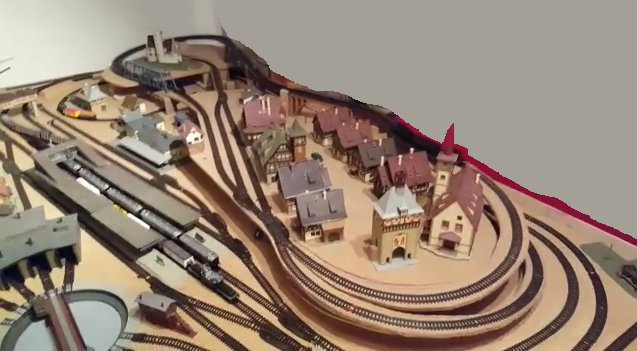
\includegraphics[width=0.5\textwidth]{img/elder_maps/anlage_papa_2019.png}
	\caption{V\"aterliche Anlage}
	\label{img:elder_maps_anlage_papa_2019}
\end{figure}

Seitdem wurde die Idee einer neuen, eigenen Anlage aufgegriffen, ohne zu wissen, wann und wie diese realisiert werden k\"onnte.
Zus\"atzlicher Spirit wurde bei einem besuchten Fahrtag des Pro Sport Berlin 24 e.V. in Berlin Wedding (zwischenzeitlich leider aufgel\"ost) getankt.
Um Weihnachten 2018 rum gab es dann eine ordentliche Instandsetzung der v\"aterlichen Anlage inklusive einiger untergeordneter Gleisplanoptimierungen.
Der Vorsatz war seitdem dreigeteilt:
\begin{enumerate}
	\item Vorbereitung einer Computersteuerung f\"ur die analoge Anlage, inkl. Erarbeitung der hierf\"ur erforderlichen elektrotechnischen Grundlagen
	\item Versuchsweise Ausgestaltung des Diorama's, auch um wesentliche Kenntnisse f\"ur eine sp\"atere Umsetzung des Eigenentwurfs zu erwerben
	\item Review des eigenen Entwurfs
\end{enumerate}
Der Eigenentwurf brachte sogar eine Aufstellung der Anlage beim Vater selbst ins Spiel (allerdings nie in R\"ucksprache...), wodurch ein Anschluss zur v\"aterlichen Anlage angedacht wurde.
Der Name der Stadt, die im Zentrum des Eigenentwurfs steht, war bereits \hl{2015} auf Granitz fixiert worden, eine fiktive Stadt in Brandenburg, wahrscheinlich s\"ud\"oestlich von Berlin Richtung Cottbus gelegen.

Wieder ein Jahr sp\"ater wurde der Eigenentwurf nochmals \"uberarbeitet und viel mit dem Bruder diskutiert.
Durch ein sich ergebendes Zeitfenster ohne berufliche und pers\"onliche Dauerauslastung wurde dann im Januar 2020 der Entschluss gefasst:
Granitz soll umgesetzt werden, egal ob mit oder ohne Platz in der Wohnung.
Durch die eigene Arbeit in der Programmierung stark von Modularisierung gepr\"agt, wurden auch verschiedene Ideen f\"ur eine Segmentierung des Eigenentwurfs durchgesponnen, um die Anlage schnell verstauen zu k\"onnen und verl\"asslich wieder zusammensetzen zu k\"onnen.

Ein weiterer - nat\"urlich v\"ollig unsinniger xD - Schritt zur Forcierung des Unterfangens war der Ankauf von Zugmaterial f\"ur das geplante Szenario.
Ganz nach dem unkonventionellen Motto: Investieren, um Argumente gegen einen schnellen Wiederausstieg zu schaffen.
Oder noch einfacher: Fakten schaffen.
Letzteres wurde mit der gegebenen Vorsicht auch bei der Ehefrau bzgl. des ben\"otigten Platzbedarfs gemacht.
Der Widerstand fiel hier aber quasi aus ...einer von vielen Gr\"unden, weshalb ich mich gl\"ucklich sch\"atzen kann, sie gefunden zu haben.



\subsection{Epoche V und Brandenburg als Thema}
\label{sec:theme}

Die Erinnerungen an die ersten Jahre nach der Wende und damit auch immer h\"aufiger werdenden Ausfl\"uge ins ehemalige Ostberlin oder umgebende Brandenburg haben bis heute einen tiefen Eindruck hinterlassen:
Von Anfang an war das f\"ur ein Kind gew\"ohnungsbed\"urftig und erschien auch etwas altbacken.
In den ersten zehn Jahren hat sich das meiner Meinung nach drastisch gewandelt, so dass das Stra{\ss}enbild in der ehemaligen DDR eher durch Relikte unterscheidbar ist.
Ein sehr junges Beispiel hierf\"ur sei in Abb.~\ref{img:inspiration_babelsberg_ambivalent} aufgezeigt:
die nahezu provisorisch anmutend gepflasterte Stra{\ss}e im R\"ucken des Schlosses Babelsberg, seinerseits ein Prunkbau.
Dass es solche Ansichten auch im Jahr 2020 und somit drei Jahrzehnte nach der Wende gibt, freut den Autor sehr.

\begin{figure}[h]
\centering
	\begin{subfigure}[b]{0.49\textwidth}
    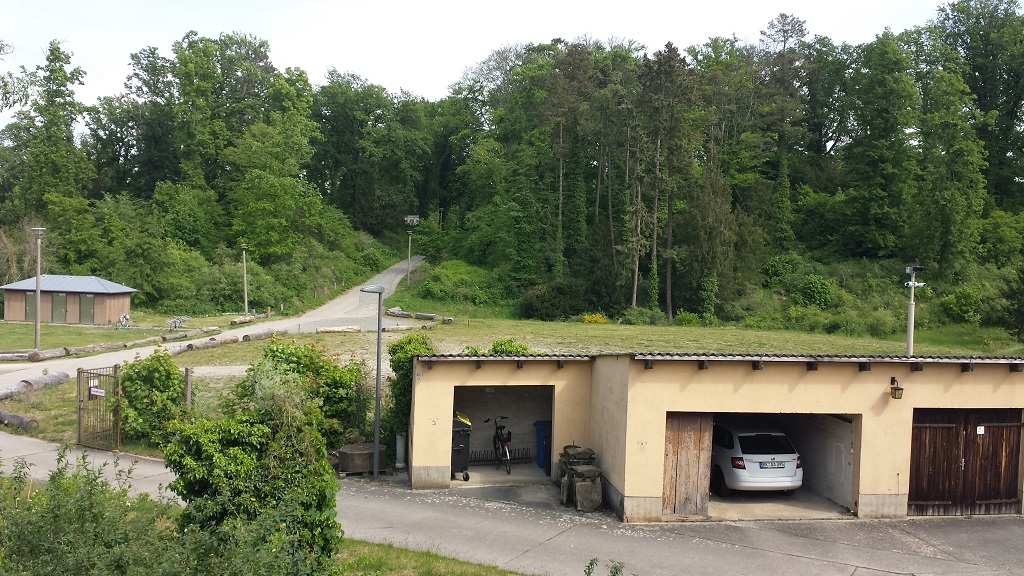
\includegraphics[width=1.0\textwidth]{img/inspiration/babelsberg_ambivalent_1.jpg}
   \caption{Links im Hintergrund die angesprochene, kopfstengepflasterte Stra{\ss}e, am Rand inzwischen mit Asphalt erweitert, und die typischen alten Laternen}
    \label{img:inspiration_babelsberg_ambivalent_1}
    \end{subfigure}
	\begin{subfigure}[b]{0.49\textwidth}
    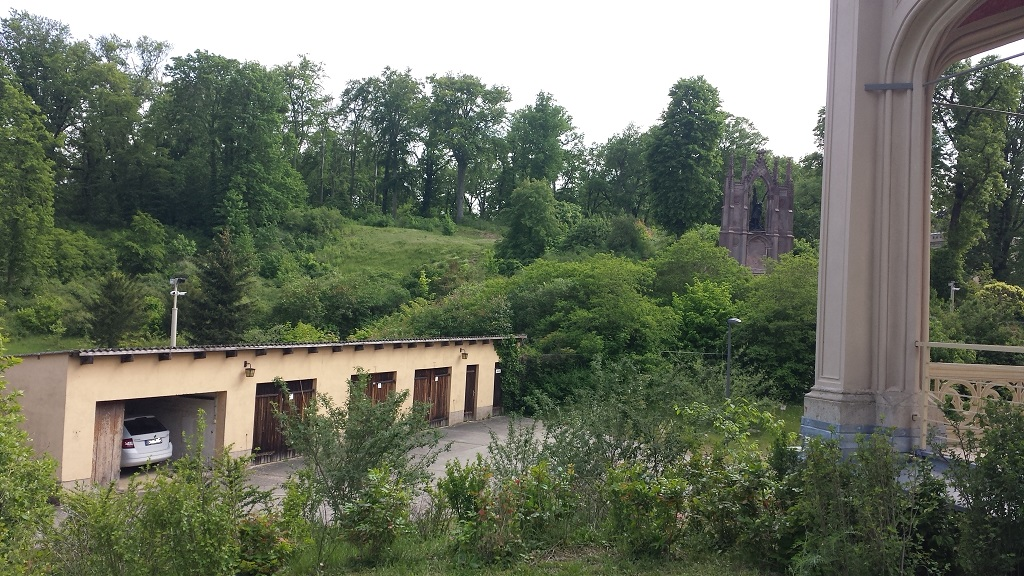
\includegraphics[width=1.0\textwidth]{img/inspiration/babelsberg_ambivalent_2.jpg}
   \caption{Die ollen Garagen schlie{\ss}en direkt an das Schloss Babelsberg an}
    \label{img:inspiration_babelsberg_ambivalent_2}
    \end{subfigure}
	\caption{Schlosspark Babelsberg: Prunkbau meets postsozialistische Nebenstra{\ss}e}
	\label{img:inspiration_babelsberg_ambivalent}
\end{figure}

Die Schw\"ache f\"ur's baldowern im Berliner Umland sowie der Reiz des Verfalls wurde bereits in Kap.~\ref{sec:author} eingef\"uhrt.
Tats\"achlich geh\"oren dar\"uber hinaus - wenngleich total amateurhaft und anspruchsarm - die Fotografie von Street Art und eben \"uberwucherten, einst\"urzenden Industrie-, Milit\"ar- und Bahnanlagen zu den seelischen Leidenschaften des Autors.
Die Absurdit\"at, d.h. der fr\"uhere Bedarf an all diesen Anlagen contra der gegenw\"artigen Aufgabe all dieser, hat f\"ur mich ein besonderes Flair.
Wo bis vor 30 Jahren noch Getummel auf blanken Betonfl\"achen stattfand, Boden fahrl\"assig verseucht wurden (\"ein Tropfen ist nichts\" ...ich war auch mal bei der Bundeswehr und wei{\ss} das), erobert sich die Natur heute ihren Platz.
(Okay, die B\"oden bleiben dennoch verseucht.)

Brandenburg ist von diesem Verfall nat\"urlich ganz besonders betroffen.
Und gleichzeitig hatten die neuen Bundesl\"ander ganz einfach und verst\"andlicherweise ihre Probleme nach der Wende.
Die Stadtflucht ist nur ein Beispiel.
Warum soll man den Ist-Zustand also nicht darstellen d\"urfen?

Der Autor versucht das mit Granitz.

Dementsprechend ist das Szenario auch sehr gut in Epoche V aufgehoben.
Das umfasst sowohl den Zeitraum unmittelbar um den Falls des Eisernen Vorhangs herum, in der Deutschen Bahnlandschaft also durch die Reichsbahn (DR) auf Ostseite und Bundesbahn (DB) auf Westseite sowie ihre Zusammenf\"uhrung in die DB AG (DBAG) gepr\"agt.
Der vielf\"altige, bunte Wagenpark und die Lackierungs\"anderungen sind wahrscheinlich einmalig in der Geschichte der Bahn.
Im Granitz um die Wende herum haben deshalb sowohl dunkel- als auch mintgr\"une Sputniks Platz, gezogen von dunkel- oder orientroten Loks der DR BR 243 Familie.
Interregio (IR) und Intercity (IC) Z\"uge werden vorwiegend in Pastelllackierung gesehen, k\"onnen aber noch Wagenmaterial aus Epoche IV enthalten.
Zugleich entspricht die fr\"uhe Epoche V - oft auch als Va bezeichnet - nat\"urlich dem Stand, auf dem ich die Deutschen Bahnen in meiner Kindheit kennengelernt habe.
Gleichzeitig bringe ich aus den alten Eigenbest\"anden auch etwas passendes Zugmaterial mit, sehr passend also.

Das sp\"atere Granitz ist dann nicht mehr so h\"aufig frequentiert.
Dies soll ebenfalls im Diorama veranschaulicht werden, ggf. durch den Austausch kleinerer Dioramaplatten.

Im Zusammenhang mit der Entscheidung f\"ur Epoche V muss ehrlicherweise aber auch ein sehr banaler Grund Erw\"ahnung finden.
Wie gesagt, hat die Epoche meine Kindheit und Jugend gepr\"agt, in diesem Sinne also auch vorgegeben, wie ein Zug aussehen muss.
Ganz ma{\ss}geblich waren dabei auch drei Familienurlaube auf Sylt mit vielen Ausblicken auf den Hindenburgdamm.
Tolle Erlebnisse!

Mein Vater konnte f\"ur Epoche V Zugmaterial nicht mehr viel Leidenschaft aufbringen.
Mein Neffe hat einen Epoche VI IC, den ich pers\"onlich absolut geschmacklos finde.
Das ist aber normal!
Wir nehmen vorwiegend die Eindr\"ucke unserer jungen Jahre mit, die sich dann ggf. noch etwas erweitern k\"onnen.
Ich selbst kann noch viel mit Epoche IV anfangen, aber \"alteres Material l\"asst den Funken kaum \"uberspringen.


\subsection{Geschichtlicher Abriss der Stadt Granitz}
\label{sec:storyOfGranitz}

Granitz war sicherlich niemals der Nabel der Welt.
Im Freistaat Preu{\ss}en eine Kleinstadt, wurde es irgendwann mit dem repr\"asentativen Bahnhofsgeb\"aude ausgestattet.
Es siedelte sich etwas Industrie an - Werkzeugmachereien, Produktion von Gebrauchsgegenst\"anden.
Die Kohlegebiete in der Lausitz sind nicht weit entfernt.
Damit knackte es auch irgendwann die Einwohnerzahl, um als echte Stadt bezeichnet zu werden.
Wie gro{\ss} diese Zahl ist, soll hier nicht diskutiert werden.

Im Zweiten Weltkrieg hat die Stadt nat\"urlich etwas Schaden abbekommen, wurde aber bei weitem nicht in Schutt und Asche zerlegt.
Warum auch?
Der Sozialismus hat dann allerdings seinen Stempel aufgepr\"agt.
Aus diesem Grund geh\"ort die Platte in das Stra{\ss}enbild, egal ob man es mag oder nicht.
Das alte Bahnhofsgeb\"aude hat sich als Zeitzeuge einer aufstrebenden Zeit erhalten.

Schlecht ging es zu DDR Zeiten aber beileibe nicht.
Insbesondere die Verkehrslage an der Haupstrecke zwischen Berlin und Dresden gelegen war gut und ist bis heute ein Grund, weshalb die Stadt nicht v\"ollig aufgegeben wurde.
Die G\"uterverkehrsanlagen am Granitzer Hauptbahnhof (heute einfach: Granitz) wurden nicht nur von den ans\"assigen Betrieben genutzt, sondern dienten auch als Umschlagplatz f\"ur den \"uberregionalen St\"uckgutverkehr.
Regionaler Pendelverkehr war und ist etabliert.
Bis Mitte der 90er waren auch viele t\"agliche Fernverkehrsverbindungen in den IR und (seltener) IC Netzen gelistet.
Der ICE hat hier nat\"urlich keinen Regelhalt, sondern f\"ahrt \"ublicherweise nur durch.
Der Autor hofft seit jeher auf einen Halt des Berlin-Warschau-Expresses, wei{\ss} aber, dass dieser Umweg unn\"otig und somit unwirtschaftlich w\"are.

Viele der stadtans\"assigen Betriebe wurden von der Treuhand einfach nur abgewickelt.
Dies geht seit den 90ern mit dem industriellen und somit auch erwerbsm\"a{\ss}igen Niedergang der Stadt und ihrer B\"urger einher.
in den sp\"aten 2000ern hat sich die Stadt ebenso wie andere St\"adte Brandenburgs etwas gefangen.
Trotzdem haftet inzwischen ein Verfall der Bahninfrastruktur und nat\"urlich auch gesellschaftlicher Liegenschaften und Wohnquartieren an.

Die von Granitz abzweigenden Nebenstrecken sind nur noch schwach frequentiert.
Dazu geh\"oren:
\begin{itemize}
	\item Die lokale Nebenstrecke zu eingemeindeten Stadtteilen: \textbf{Granitz} $\rightarrow$ \textbf{Sch\"onblick} $\rightarrow$ \textbf{Granitz-Walddorf} (s\"ud\"ostlich vom Zentrum)
	\item Die direkte Nebenstrecke zur n\"achsten, etwa gleich gro{\ss}en, s\"udwestlich gelegenen Stadt Schattenwalde: \textbf{Granitz} $\rightarrow$ \textbf{Schattenwalde}
	\item Die Nebenstrecke \"uber die westlich gelegenen D\"orfer verzeichnete bis zum Ende der 90er noch einen schwachen RB-Betrieb, wurde aber inzwischen stillgelegt.
\end{itemize}


\subsection{Ein Wort zum Thema Genauigkeit und Konsistenz}
\label{sec:modelingAccuracy}

Der Autor hat einige Schw\"achen, was die finale Detailg\"ute alle seiner Arbeiten betrifft.
Das Hauptinteresse liegt vielmehr auf allgemeinen und abstrakten Darstellungen.
Mit dieser Modellbahnanlage wird das schon weit aufgebrochen.

Zur Genauigkeit kann in vieler Hinsicht Kritik erfolgen:
\begin{itemize}
	\item Feinheit im Diorama,
	\item Realismus im betrieblichen Ablauf,
	\item diesbez\"uglich also auch im Gleisplan,
	\item Exaktheit in der Verwendung des Zugmaterials, sowohl was die Kombination von Loks und Wagen als auch die zeitlich korrekte Einordnung erfolgt, sowie
	\item Konsistenz des Szenarios im allgemeinen.
\end{itemize}

Dies alles kann und werde ich nicht zu 100~\% einhalten.
Grund daf\"ur ist die Bandbreite der Epoche V auf der einen Seite und die eigene Schludrigkeit auf der anderen Seite.
Modellbahn super realistisch zu machen, das schaffen sicherlich nur die allerwenigsten.
Zu meckern gibt es immer.
Aber am Ende bleibt es ein Hobby und mein Szenario enth\"alt nun mal auch viel Fiktion.
Ich folge keinem Anspruch, dem ich nicht gerecht werden kann und will.

Zweieinhalb kurze Beispiele, die man in Granitz beobachten wird:
\begin{itemize}
	\item[1:] Der Vorsatz, das Granitz in den fr\"uhen 90ern sowie die ver\"anderte Situation zwanzig Jahre sp\"ater darzustellen, wird nicht vollst\"andig durch Dioramatausch realisierbar sein.
	Einige Elemente in der Szene werden entweder schwarz oder wei{\ss} sein.
	Alles andere st\"o{\ss}t an meine Grenze der Praktikabilit\"at bei einem Privatprojekt.
	\item[2:] Die verschiedenen, zeitlich zu differenzierenden Lackierungen der in Granitz im Fokus stehenden BR 243 Familie sowie der angeh\"angten Doppelstockwaggons werden potenziell gemischt im Fahrbetrieb anzutreffen sein.
	Es macht keinen Sinn, jede Lackierungsform der Lok und auch nicht die Zuschreibung zu DR, DB oder DBAG in zwei- bis dreifacher St\"uckzahl vorzuhalten.
	Das Geld kann anders sinnvoller investiert werden und - Realismus beiseite geschoben - der Fahrbetrieb wird auf diese Weise bunter und durchmischt die Zeiten.
	\item[2.5:] In Erg\"anzung zum vorherigen Punkt ist es mir pers\"onlich auch nicht so wichtig, ob in Brandenburg nun typischerweise eine BR 112 oder BR 114 vor Regionalbahnen gespannt wird.
	Dieser Unterschied ist f\"ur mich marginal.
	Ich wei{\ss}, dass andere dort drau{\ss}en anders denken und respektiere das; hier muss der Besucher aber damit leben.
\end{itemize}

Auf der anderen Seite sind Kritiker eingeladen, mir in puncto Begrifflichkeit dort wo notwendig auf die Finger zu hauen.
Hier lerne ich gern dazu bzw. lasse mich auf Schludrigkeiten hinweisen, denn Begrifflichkeit ist zum Schluss der Schl\"ussel f\"ur ein gutes Gesamtverst\"andnis der Dokumentation.
Ein kleiner Beweis:
Das Wort Modul verwende ich h\"aufig im Beruf, habe mich aber schnell dazu gezwungen, im Modellbahnkontext streng zwischen Segment und Modul (als etwas wie auch immer, ab Vereinsebene aufw\"arts genormtes Segment) zu differenzieren.
Im Softwareteil (Kap.~\ref{sec:software}) findet bzgl. der Terminologie aber ein Kontextwechsel statt, also aufgepasst!